%%%%%%%%%%%%%%%%%%%%%%%%%%%%%%%%%%%%%%%%%
% Stylish Article
% LaTeX Template
% Version 2.2 (2020-10-22)
%
% This template has been downloaded from:
% http://www.LaTeXTemplates.com
%
% Original author:
% Mathias Legrand (legrand.mathias@gmail.com) 
% With extensive modifications by:
% Vel (vel@latextemplates.com)
%
% License:
% CC BY-NC-SA 3.0 (http://creativecommons.org/licenses/by-nc-sa/3.0/)
%
%%%%%%%%%%%%%%%%%%%%%%%%%%%%%%%%%%%%%%%%%

%----------------------------------------------------------------------------------------
%	PACKAGES AND OTHER DOCUMENT CONFIGURATIONS
%----------------------------------------------------------------------------------------

\documentclass[fleqn,10pt]{SelfArx} % Document font size and equations flushed left

\usepackage[spanish]{babel} % Specify a different language here - english by default
\usepackage{apalike}
\usepackage{comment} % Allows us to comment parts out of the code.
%----------------------------------------------------------------------------------------
%	COLUMNS
%----------------------------------------------------------------------------------------

\setlength{\columnsep}{0.55cm} % Distance between the two columns of text
\setlength{\fboxrule}{0.75pt} % Width of the border around the abstract

%----------------------------------------------------------------------------------------
%	COLORS
%----------------------------------------------------------------------------------------

\definecolor{color1}{RGB}{0,0,90} % Color of the article title and sections
\definecolor{color2}{RGB}{0,20,20} % Color of the boxes behind the abstract and headings

%----------------------------------------------------------------------------------------
%	HYPERLINKS
%----------------------------------------------------------------------------------------

\usepackage{hyperref} % Required for hyperlinks

\hypersetup{
	hidelinks,
	colorlinks,
	breaklinks=true,
	urlcolor=color2,
	citecolor=color1,
	linkcolor=color1,
	bookmarksopen=false,
	pdftitle={Title},
	pdfauthor={Author},
}

%----------------------------------------------------------------------------------------
%	ARTICLE INFORMATION
%----------------------------------------------------------------------------------------

\JournalInfo{Introducción a la Astronomía} % Journal information
\Archive{Noviembre de 2020} % Additional notes (e.g. copyright, DOI, review/research article)

\PaperTitle{Características de cuerpos estelares en la región central de la Vía Láctea} % Article title

\Authors{Rudik Rompich\textsuperscript{1}*, Baptiste Bauer\textsuperscript{1}**} % Authors
\affiliation{\textsuperscript{1}\textit{Departamento de Física, Universidad del Valle de Guatemala, Guatemala}} % Author affiliation
\affiliation{\,*\textbf{Correo de contacto}: rom19857@uvg.edu.gt}
\affiliation{**\textbf{Correo de contacto}: bau171501@uvg.edu.gt}
% Corresponding author

\Keywords{Cuerpos estelares --- Centro de la Vía Láctea --- Infrarojo cercano} % Keywords - if you don't want any simply remove all the text between the curly brackets
\newcommand{\keywordname}{Keywords} % Defines the keywords heading name

%----------------------------------------------------------------------------------------
%	ABSTRACT
%----------------------------------------------------------------------------------------

\Abstract{Analizamos las características de dos cuerpos estelares presentes en la región del centro de la Vía Láctea. Las imágenes fueron tomadas en el infrarrojo cercano En base a los datos reportados en el catálogo de \textit{Two Micron All-Sky Survey (2MASS)} y medidos por el satélite Gaia, presentamos para las dos estrellas sus coordenadas, colores, temperaturas, disctancias, luminosidades, flujos, tamaños, tipos espectrales, clases espectrales y sus ubicaciones en el diagrama HR. Una parte de estos resultados decaen del supuesto que los cuerpos estudiados son estrellas de la secuencia principal del diagrama de Hertzsprung-Russell.}

%----------------------------------------------------------------------------------------

\begin{document}

\maketitle % Output the title and abstract box

%\tableofcontents % Output the contents section

\thispagestyle{empty} % Removes page numbering from the first page
%----------------------------------------------------------------------------------------
%	ARTICLE CONTENTS
%----------------------------------------------------------------------------------------

\section*{INTRODUCCIÓN}\label{sec:intro}
\addcontentsline{toc}{section}{INTRODUCCIÓN}
Al observar el cielo, podemos encontrar mucha información acerca de lo que podemos ver. El telescopio Gaia ha completado los diferentes catálogos de estrellas con informaciones extensas, que podemos usar para predecir las características de las estrellas observables con un telescopio profesional. El objetivo de este trabajo es demostrar el alcance del posible análisis de las características de un cuerpo estelar partiendo de muy poca información.
 
\section*{MUESTRA}\label{sec:muestra}

\addcontentsline{toc}{section}{MUESTRA}
\begin{figure}[ht]
    \centering
    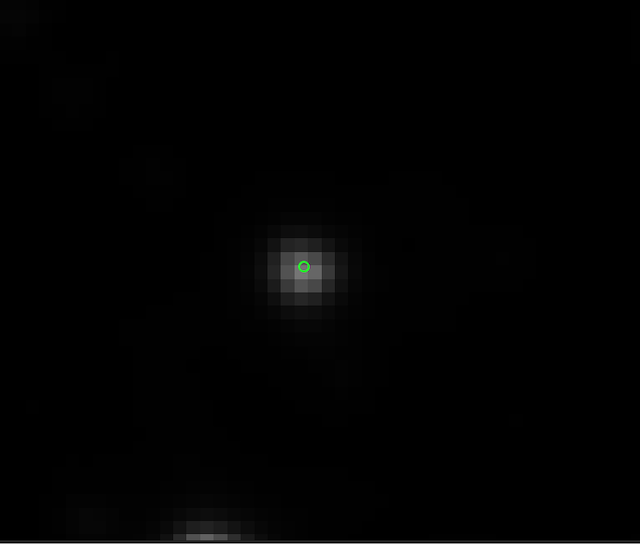
\includegraphics[scale=0.35]{Imagenes/Rudik-1.png}
    \caption{IGRF17451}
    \label{fig:estrella-rudik}
\end{figure}
\begin{figure}[ht]
    \centering
    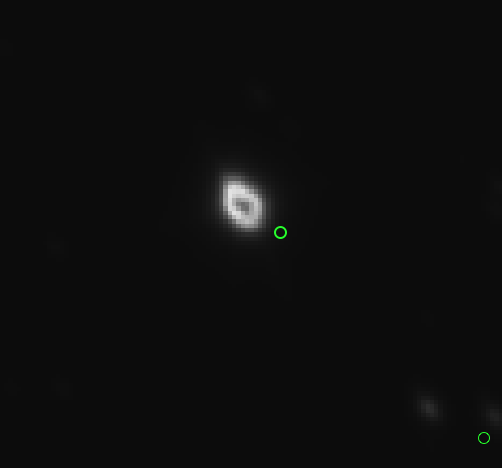
\includegraphics[scale=0.4]{Imagenes/Baptiste-1.png}
    \caption{MAXIJ1543}
    \label{fig:estrella-bapt}
\end{figure}

% Please add the following required packages to your document preamble:
% \usepackage{booktabs}
\begin{table*}[t]
\caption{}
\label{tab:estrellas}
\begin{tabular}{@{}lllllllllll@{}}
\toprule
Imagen     & \begin{tabular}[c]{@{}l@{}}Coordenadas \\ ecuatoriales\end{tabular}       & Color   & \begin{tabular}[c]{@{}l@{}}Tempe-\\ ratura\end{tabular} & \begin{tabular}[c]{@{}l@{}}Distancia\\ (m)\end{tabular} & \begin{tabular}[c]{@{}l@{}}Lumino-\\ sidad (W)\end{tabular} & \begin{tabular}[c]{@{}l@{}}Flujo     \\ (W/m²)\end{tabular} & Tamaño & \begin{tabular}[c]{@{}l@{}}Tipo \\ Espectral\end{tabular} & \begin{tabular}[c]{@{}l@{}}Clase \\ Lumi-\\ nosidad\end{tabular} & \begin{tabular}[c]{@{}l@{}}Posición \\ (HR)\end{tabular} \\ \midrule
IGRFJ17451 & \begin{tabular}[c]{@{}l@{}}Ra: 266.232544\\ Dec: -30.390377\end{tabular}  & 5.06E-7 & 5778                                                    & 3.112 E19                                               & 0.994                                                       & 3.1 E-14                                                    & 0.99   & G2                                                        & V                                                                & MS                                                       \\
MAXIJ1543  & \begin{tabular}[c]{@{}l@{}}Ra:  235.955621\\ Dec: -56.440075\end{tabular} & 3.62E-7 & 8000                                                    & 1.97E19                                                 & 2.59                                                        & 2.0E-13                                                     & 0.8385 & K II                                                        & V                                                                & MS                                                       \\ \bottomrule
\end{tabular}
\end{table*}


\begin{table}[t]
\caption{}
\label{tab:estrellas2}
\begin{tabular}{@{}lllll@{}}
\toprule
Imagen     & Instrumento & Fecha de observación & Filtro &  \\ \midrule
IGRFJ17451 & LIRIS       & 9 de abril 2015      & $K_s$   &  \\
MAXIJ1543  & HAWK-I      & 10 de abril 2018     & H      &  \\ \bottomrule
\end{tabular}
\end{table} 
\section*{METODOLOGÍA}\label{sec:analisis}
\addcontentsline{toc}{section}{METODOLOGÍA}


Primero se determinarón las coordenadas ecuatoriales y la magnitud aparente de la estrellas dadas por el \textit{software SAOImageDS9} extraídas de las Figuras \ref{fig:estrella-rudik} y \ref{fig:estrella-bapt} proporcionadas por \cite{lopez2019quiescent}.\\

Con las coordenadas ecuatoriales, se busca el paralaje en la página oficial del telescopio Gaia (Gaia Archive). \footnote{\url{https://gea.esac.esa.int/archive/}}\\
\begin{align}
    d&=\frac{1}{p}\\
    p&=\text{paralaje}*10^{-3}
\end{align}
De \cite{lol:cohen2003spectral}, sabemos que la longitud de onda central de la banda K$_s$, en la cual se realizó la medición, es de $\lambda=2.159\mu m$, además que la densidad de flujo es de $F_x^0=4.283Wcm^{-2}\mu m^{-1}$. Para obtener el flujo, multiplicamos a la densidad de flujo por $\lambda$: al convertir las unidades a las estándares del Sistema Internacional, $\lambda F_x^0=9.4226*10^{-10} Wm^{-2}$. Encontramos el flujo: 
\begin{align}
    m_x=-2.5\log_{10}\left(\frac{F_x}{F_x^0}\right) \Rightarrow F_x=F_x^0 10^{-\frac{m_x}{2.5}}
\end{align}
\begin{align}
    F_x= 9.4226*10^{-10}*10^{-\frac{11.202}{2.5}}=3.114*10^{-14} W/m^2
\end{align}
Con el flujo, podemos encontrar la luminosidad aparente:
\begin{align}
    L=F*A=F*4\pi W
\end{align}
Se sabe que $=L_\odot=3.828*10^{26}$W:
\begin{align}
    \text{Luminosidad comparado al sol}=\frac{L}{L_\odot}
\end{align}

La luminosidad de la estrella nos da un valor específico \textit{x} veces mayor o menor a la del Sol. Si asumimos su posición en el diagrama de Hertzsprung-Russell, se estima que la temperatura de la estrella debe ser de  cierta cantidad de Kelvins. 
\begin{align}
    T = \text{temperatura supuesta } K 
\end{align}

Con este dato, podemos encontrar al radio de la estrella: usamos a la ley de radiación de un cuerpo negro:
\begin{align}
    F=\frac{L}{A}=\frac{L}{4\pi R^2}=\sigma T^4
\end{align}

\begin{align}
    R=\sqrt{\frac{L}{4\pi \sigma T^4}}m
\end{align}

Se sabe que el radio del Sol es $R_\odot=696340*10^3$m
\begin{equation*}
    \text{Radio comparado al sol}=\frac{R}{R_\odot}
\end{equation*}

Con la temperatura, también podemos encontrar el color de la estrella: en donde $b=2.897771955*10^{-3}$mK.
\begin{align}
    \lambda_{max}=\frac{b}{T}
\end{align}

Para el cálculo de las propiedades de las estrellas fue necesario desarrollar un código que fue alojado en Github\footnote{\url{https://github.com/RudiksChess/Astronomy_Presentations/blob/main/Calculos.ipynb}}. 
\section*{RESULTADOS}\label{sec:resultados}
\addcontentsline{toc}{section}{RESULTADOS}

Como se aprecia en el Cuadro \ref{tab:estrellas2} las imágenes IGRFJ17451 y MAXIJ1543 se obtuvieron de \cite{lopez2019quiescent} y luego de su respectivo análisis se obtuvo el Cuadro \ref{tab:estrellas}. \\

Para la primera estrella encontrada en IFRFJI17451 (véase Figura \ref{fig:estrella-rudik}) se determinó, por la suposición que se hizo, que la estrella tiene 0.99 $R_{\odot}$ y una luminosidad de 0.994 $L_{\odot}$ lo que la hace una estrella prácticamente igual al sol. Su tipo espectral es G2 y su clase de luminosidad es V. Su posición en el diagrama HR está en la secuencia principal. Es decir, una enana amarilla. \\

La zona habitable de está estrella, según \cite{lissauer_2020}, estaría entre 0.9 UA a 1.5 UA (al ser prácticamente igual al Sol). Lo que haría a la estrella potencialmente propensa a albergar vida, con las condiciones correctas de sus planetas que la orbitan. Por otro lado, los planetas que podría albergar esta estrella (basado las características del sol) serían gigantes gaseosos; los cuales podrían ser detectados por el método de imagen directa, tal y como se explica en \cite{bohn2020two}, en donde estudiaron un planeta similar al sol en el cual orbitan dos gigantes gaseosos.  \\

De la misma forma, para la estrella estudiada en MAXIJ1543, mostrada en la figura \ref{fig:estrella-bapt}, se estimó un radio de $0.8385 R_\odot$ y una luminosidad de $2.60 L_\odot$. La clasificación correspondiente sería K II. Como lo hemos supuesto, esta estrella pertenece a la secuencia principal. \\

Ya que esta estrella es más brillante y más caliente que el Sol, la zona habitable será un poco más lejos que la que existe alrededor de nuestra estrella. En unidades astronómicas (AU), se estima que iría de 0.95 AU hasta 1.676 AU. 
Ya que R=$0.8385 R_\odot$, se realizó una gráfica comparando los radios de las estrellas vs las masas de los planetas que los orbita.
\begin{figure}[ht]
    \centering
    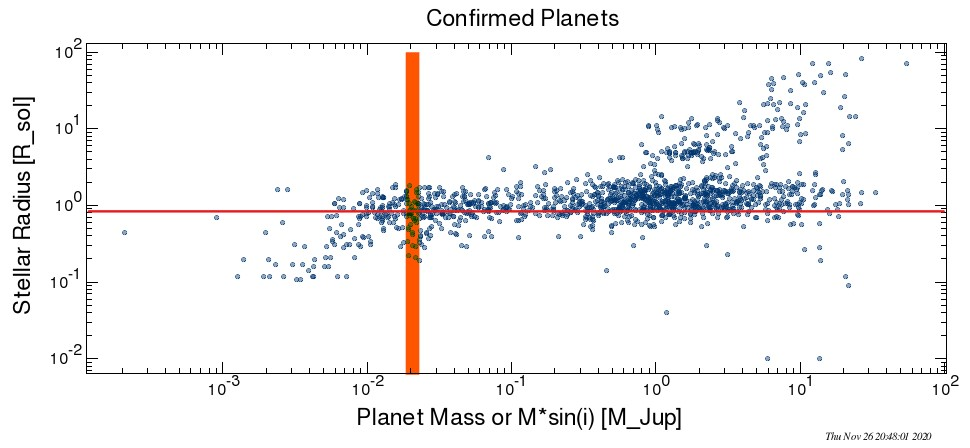
\includegraphics[scale=0.35]{Secciones/Radios.jpg}
    \caption{Radios estelares vs Masas de los planetas orbitando. }
    \label{fig:radios}
\end{figure}
En la Figura \ref{fig:radios}, obtenida de \cite{iceplotter_2020}, existen dos líneas: la horizontal indica la masa estimada de la estrella \ref{fig:estrella-bapt}. La línea vertical separa arbitrariamente los planetas con masas comparable a la de la Tierra (a la izquierda) y los planetas con masas comparables a la de Júpiter (a la derecha). Notamos que existen planetas comparables tanto a la Tierra como a Júpiter en la línea horizontal. A pesar de existir más planetas del tipo de Júpiter en la gráfica, podría ser un sesgo del sobreviviente: al graficar únicamente los planetas confirmados, y sabiendo de que es más fácil confirmar la existencia de planetas comparables a Júpiter, no podemos concluir nada más que puede existir cualquier clase de planeta orbitando a la segunda estrella.




 
\section*{DISCUSIÓN}\label{sec:discusion}
\addcontentsline{toc}{section}{DISCUSIÓN}

La deducción presentada solo presenta confianza acerca de tres datos. En base al paralaje y la magnitud absoluta, solo fue posible encontrar a la distancia del cuerpo estelar, su luminosidad y su flujo. Con el fin de estimar subsecuentes datos, se ha tenido que realizar el supuesto que el objeto estudiado pertenece a la secuencia principal de estrellas. Así es como se pudo dar un orden de magnitud para la temperatura y así encontrar el color y el radio de la estrella estudiada. Nótese que el análisis en ningún punto es válido si la estrella llegue a no ser parte de la secuencia principal. Se recomienda, especialmente para el caso de la segunda estrella, estudiar la pertenencia a diferentes clases en el diagrama de Hertzsprung-Russell (HR).\\

Se encontró un sesgo al determinar la distancia de la estrella de la Figura \ref{fig:estrella-rudik} y que se presenta en el Cuadro \ref{tab:estrellas} ya que los datos experimentales presentaron un paralaje negativo. Este es un fenómeno poco probable, debido a la certeza del telescopio GAIA. Sin embargo, es un problema que suele estar presente en las observaciones del telescopio y no es recomendado obviarlo, por las implicaciones que podría tener en una investigación con un requerimiento elevado de precisión, como lo explica \cite{gaia2018gaia}. El artículo científico anteriormente mencionado explicaba ciertas metodologías para corregir el paralaje negativo, que se basaban en métodos complejos a simplemente usar la incertidumbre dada por el archivo de GAIA; por lo cual se decidió usar este método. Esto implica, por la poca precisión del método, que los datos obtenidos para la estrella 1 del Cuadro \ref{fig:estrella-bapt} presentan un sesgo enorme y no podrían ser considerados precisos ni confiables.  \\

Finalmente mencionamos que, luego de revisar los datos reportados por \cite{lopez2019quiescent}, se encontró que la segunda imagen no fue analizada en el filtro que fue mencionado al inicio de la realización de este trabajo. Al revisar el cuadro \ref{tab:estrellas2}, notamos que el filtro de observación para la segunda imagen fue $H$ y no $K_s$. Se recomienda revisar la procedencia de las imágenes antes de procesarlas. 
\section*{CONCLUSIONES}\label{sec:conclusiones}
\addcontentsline{toc}{section}{CONCLUSIONES}
\begin{enumerate}
    \item Se determinó que con el paralaje y la magnitud aparente de un cuerpo estelar, es posible determinar con gran exactitud la distancia, luminosidad y el flujo del objeto.
    \item Se comprobó que n base a las relaciones empíricas existentes, es posible realizar estimaciones acerca de subsecuentes características del cuerpo estudiado, como su temperatura, color y radio.
    \item Se determinó que en base a la luminosidad y al flujo de una estrella, es posible estimar su zona habitable.
\end{enumerate} 
\section*{ACKNOWLEDGEMENTS}\label{sec:acknow}
\addcontentsline{toc}{section}{ACKNOWLEDGEMENTS}

\textbf{Comentario de Rudik}\\
\indent Fue un proyecto que realmente hizo darme cuenta de varias cosas: (1) Eventualmente, en algún momento me gustaría dedicarme a realizar investigación, ya que es interesante documentarse, experimentar y presentar los resultados. (Como lo del paralaje negativo, que me hizo percatarme que incluso astrónomos de alto calibre, tenían los mismos problemas que yo y que existían algo equivale a \textit{StackOverFlow} pero para astronomía para resolver dudas). (2) Que en el futuro, la astronomía podría ser un camino bastante viable para mí (en algún momento de mi vida quizás me lo plantee más seriamente). (3) Que aunque este semestre haya sido mi último semestre en física, Introducción a la Astronomía definitivamente fue el mejor curso de física que tomé en estos dos últimos años (aunque siento que no me esforcé al 100\%, está pandemia me ha afectado demasiado) que me hizo replantearme si me decisión es la correcta. (4) Que realmente, me habría gustado que este proyecto hubiese tenido programación involucrada y análisis estadísticos; ya que en los papers en los que consulté, parece ser que la programación y la estadística son de las cosas más esenciales y que hacen que sean más enriquecedores.     \newline
\newline
\indent\textbf{Comentario de Baptiste}\\
Ese proyecto es una forma muy interesante de culminar el curso de Introducción a la Astronomía, al menos a nivel personal. Mi rama favorita de la física es la parte teórica, a contrario de Kristhell, quien es una física experimental de corazón. Cuando entré a la Universidad, la astrofísica era mi motivación. Luego de haber llevado un curso de introducción a la física de partículas, esta área se volvió mi favorita. En el momento de llevar el curso de Introducción a la Astronomía, mi visión fue de nuevo cuestionada. El curso me pareció increíble y es fascinante conocer acerca de la vida de los astrofísicos experimentales. Este proyecto, sin embargo, me volvió a asegurar que la parte experimental no me gusta. Analizar imágenes y describir objetos me parece tedioso. Si un día me encamino hacia la Astrofísica, no será en una perspectiva experimental.
 


%------------------------------------------------



%---------------------------------------------
%----------------------------------------------------------------------------------------
%	REFERENCE LIST
%----------------------------------------------------------------------------------------

\phantomsection
\bibliographystyle{apalike}
\bibliography{sample.bib}


\end{document}